%===================================== Appendices =================================

\begin{appendices}

\chapter{Board layout and 3D model}

\section{Fusion 360 3D model}
\begin{figure}[!h]
\begin{center}
\center
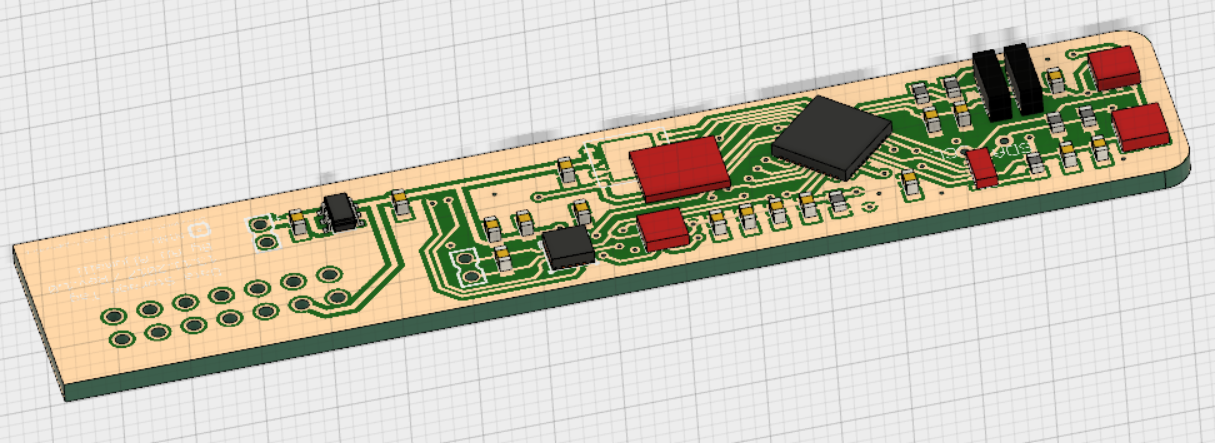
\includegraphics[scale=0.8, angle =90]{Illustrations/3D_model.png}  
\caption{Board 3D model}
\end{center}
\end{figure}

\begin{figure}[!h]
\begin{center}
\center
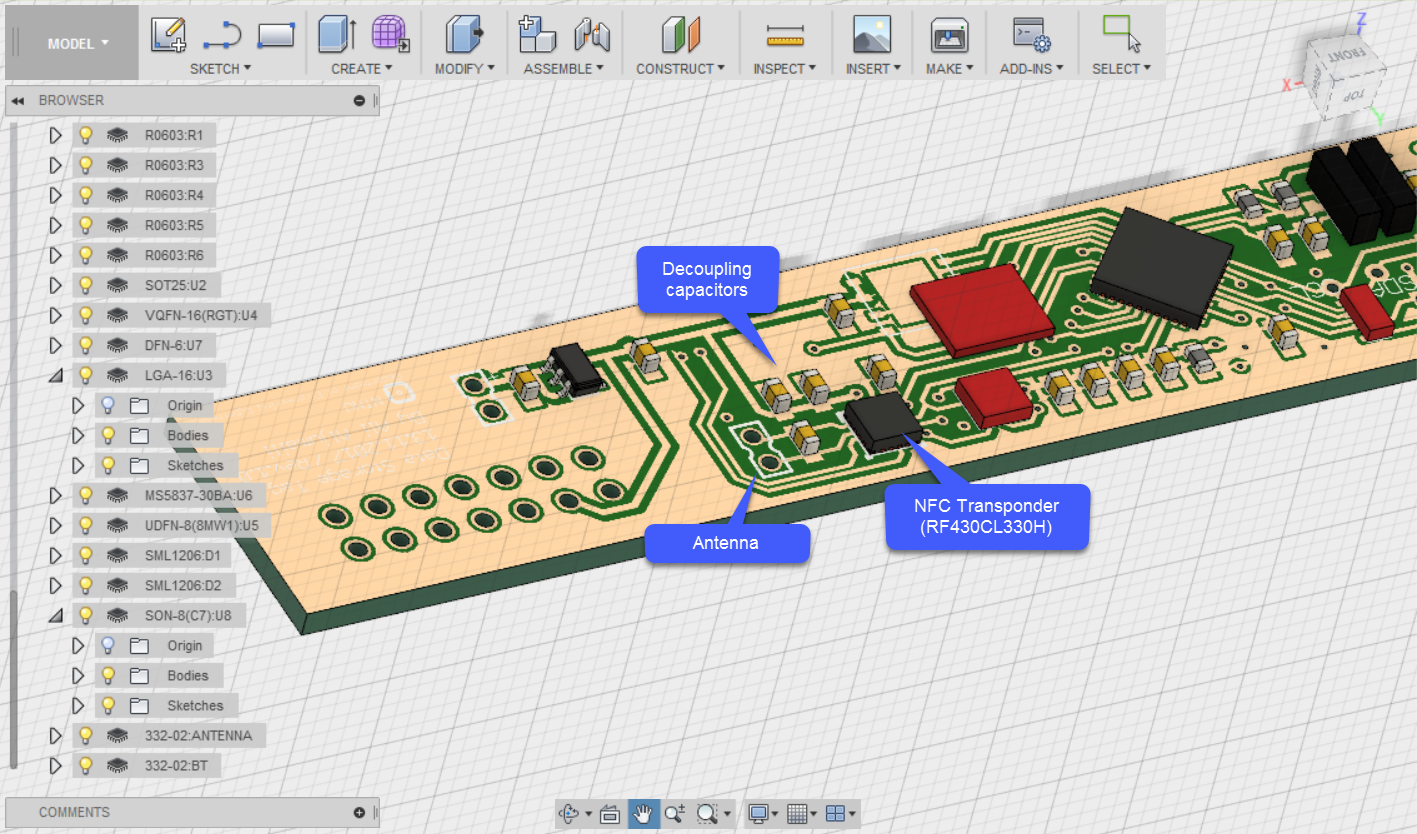
\includegraphics[scale=0.7, angle =90]{Illustrations/fusion_3d_view.png}  
\caption{Board 3D model explained}
\end{center}
\end{figure}


\section{Full schematics}
\begin{figure}[!h]
\begin{center}
\center
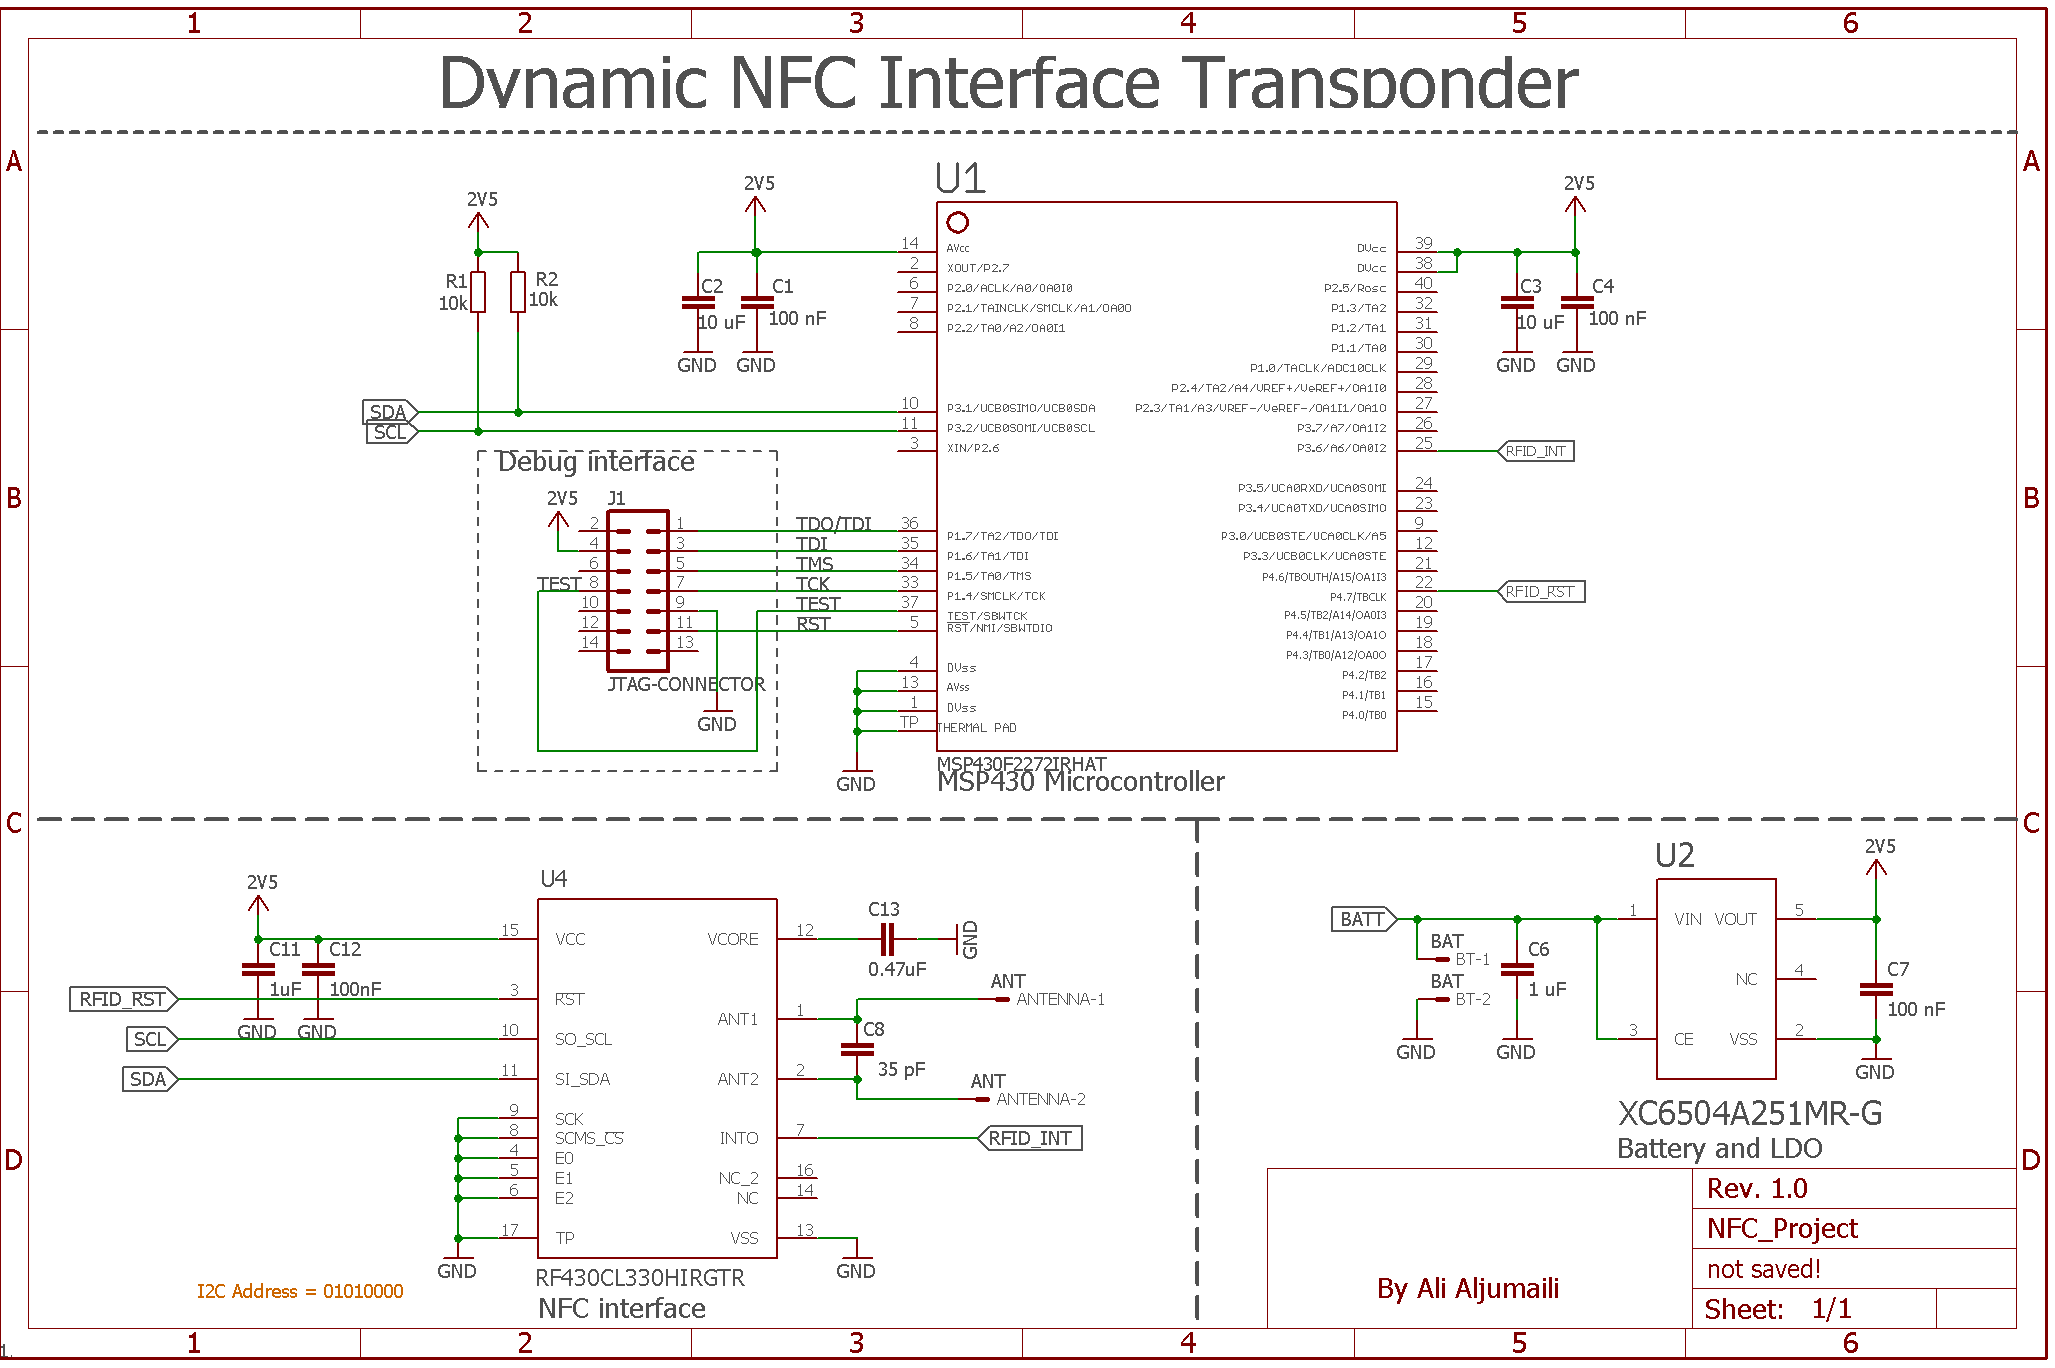
\includegraphics[scale=0.7, angle =90]{Illustrations/schematics.png}  
\caption{Full project schematics}
\label{Full_schematics}
\end{center}
\end{figure}




\section{Board layers}
\begin{figure}[h]
\begin{center}
\center
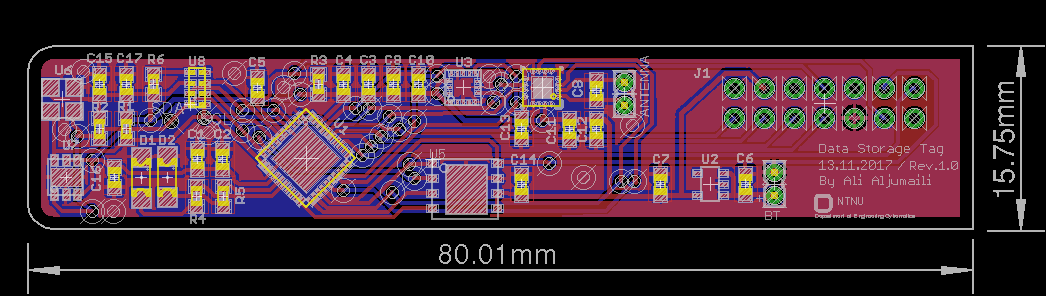
\includegraphics[scale=1.5]{Illustrations/brdscreenshot.png}  
\caption{Board layout}
\label{eagle_package}
\end{center}
\end{figure}

\pagebreak
\begin{figure}[!h]
\begin{center}
\center
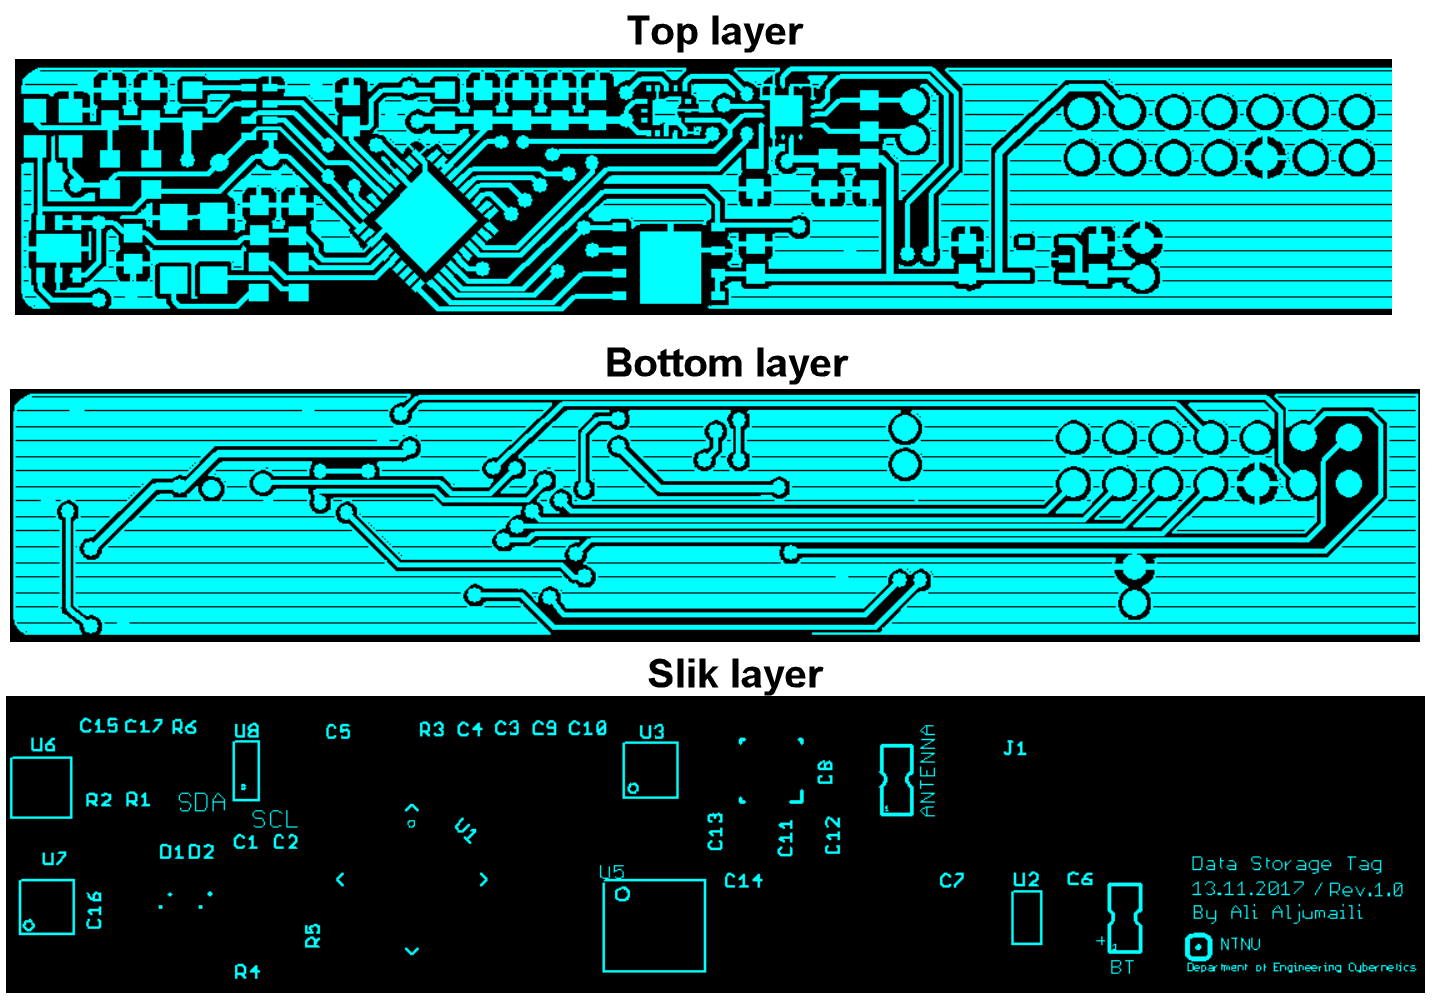
\includegraphics[scale=0.7, angle =90]{Illustrations/Board_layouts.png}  
\caption{Board layouts}
\label{board_outlines}
\end{center}
\end{figure}


\section{Produced PCB}
\begin{figure}[!h]
\begin{center}
\center
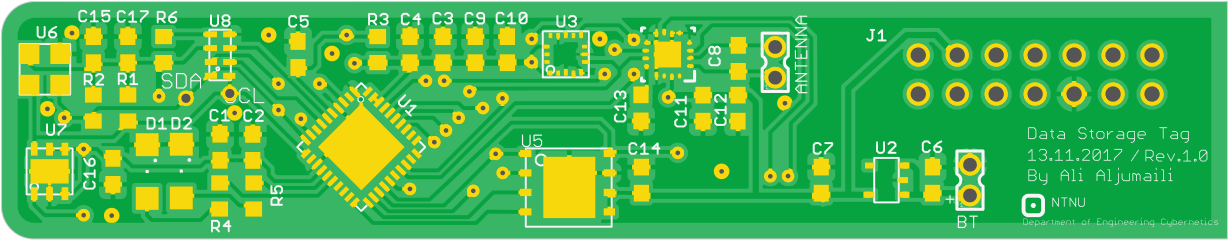
\includegraphics[scale=0.65]{Illustrations/board_layout_nice.png}  
\caption{Eagle's Board Layout}
\end{center}
\end{figure}

\begin{figure}[!h]
\begin{center}
\center
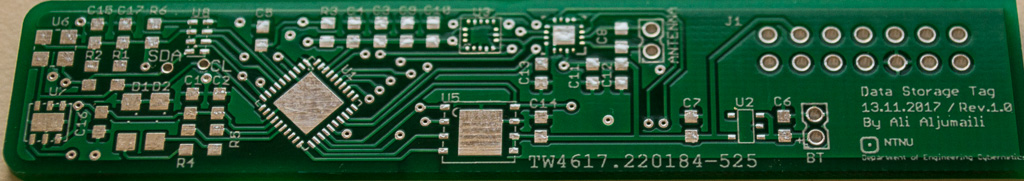
\includegraphics[scale=1.5]{Illustrations/test_prototype_front.jpg}  
\caption{PCB front}
\end{center}
\end{figure}

\begin{figure}[!h]
\begin{center}
\center
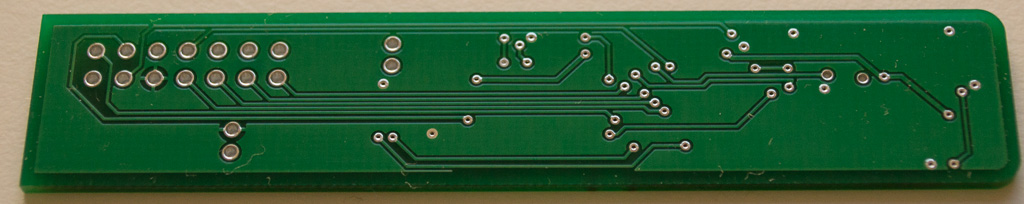
\includegraphics[scale=1.5]{Illustrations/test_prototype_back.jpg}  
\caption{PCB back}
\end{center}
\end{figure}




\chapter{Bill of Materials}

%\begin{table}[ht]
\centering
\begin{adjustbox}{width=1.2\textwidth,center=\textwidth}
\begin{tabular}{|c|c|c|c|c|c|c|}
\hline 
\rowcolor{Gray}
Item  & Qty & Designator  & Value and Description & Manufacturer & Part Number & Supplier\\  
\hline 
1 & 10 & C1,C4,C7,C9,C10, &0.1uF SMD Ceramic Capacitor & KEMET & C0603C104K5RECTU & Mouser \\ 
   &    & C12,C14,C15,C16,C17& 							  &    &  & \\ 
\hline 
2 & 2 & C2,C3 & 10 uF SMD Ceramic Capacitor & KEMET & C0603C106M9PACTU & Mouser \\ 
\hline 
3 & 2 & C6, C11 & 1 uF SMD Ceramic Capacitor & KEMET & C0603C105K8PACTU & Mouser \\ 
\hline 
4 & 1 & C8 & 35 pF SMD Ceramic Capacitor & KEMET & C0603C360J5GACTU & Mouser \\ 
\hline 
5 & 1 & C13 & 0.47 uF SMD Ceramic Capacit& TDK & CGA3E3X7R1H474K080AE & Mouser \\ 
\hline 
6 & 1 & C5 & 10 nF SMD Ceramic Capacit  & KEMET & C0603C103J5REC7411 & Mouser \\
\hline 
7 & 1 & D1 & Red SMD LED & Broadcom & HSMC-C191-T0000& Mouser \\ 
\hline 
8 & 1 & D2 & Green SMD LED & Lumex & SML-LX1206GC-TR1 & Mouser \\ 
\hline 
9 & 1 & J1 & 14P header & 3m & N2514-6002RB & Mouser \\ 
\hline  
10 & 3 & R1,R2,R6 & 10k  SMD resistor & Bourns & CR0603-FX-1002GLF & Mouser \\ 
\hline 
11 & 2 & R4,R5 & 470 & Bourns & CR0603-FX-5100ELF & Mouser \\ 
\hline 
12 & 1 & R3 & 47k & Bourns & CR0603-JW-473GLF & Mouser \\ 
\hline
13 & 1 & U1 & 16-bit MCU Ultra-Lo-pwr & Texas Instruments  & MSP430F2274IRHAT & Mouser\\ 
\hline 
14 &1  & U2  &  	LDO Voltage Regulator,	SOT-25-5 package & Torex Semiconductor & XC6504A251MR-G & Mouser \\ 
\hline 
15 & 1 & U3 &   Real Time Clock & Micro Crystal & RV-8803-C7-32.768kHz-3PPM-TA-QC & Mouser \\ 
\hline 
16 & 1 & U4 &   Accelerometers 16 bit LGA 6 degree Tri-axis Digtl Mgnt & 
Kionix & KMX62-1031-SR & Mouser\\
\hline 
17 & 1 & U5 &   DynamicNFC Interface Transponder & Texas Instruments & RF430CL330HIRGTR & Mouser \\
\hline 
18 & 1 & U6 &   Flash Memory 64Mb, SPI, UDFN-8 & Adesto Technologies & AT45DB641E-MHN-Y & Mouser \\
\hline 
19 & 1 & U7 &   Pressure Sensor & Measurement Specialties  & MS583730BA01-50 & Mouser \\
\hline 
20 & 1 & U8 &   Digital Temp Sensor High Accuracy, I2C, DFN-6 & Silicon Labs & SI7051-A20-IM & Mouser \\
\hline 
21 & 1 & Antenna & Flexible NFC antenna (13.56 MHz) & Tacoglas & FXR.06.A & Mouser  \\ 
\hline 
22 & 1 & Antenna & Flexible NFC antenna (13.56 MHz) & Tacoglas & FXR.07.A & Mouser \\ 
\hline 

\end{tabular} 
 \label{tb:BOM}
\end{adjustbox}

%\end{table}

\chapter{Project work breakdown}

\section{Work breakdown structure}
\begin{figure}[h]
\begin{center}
\center
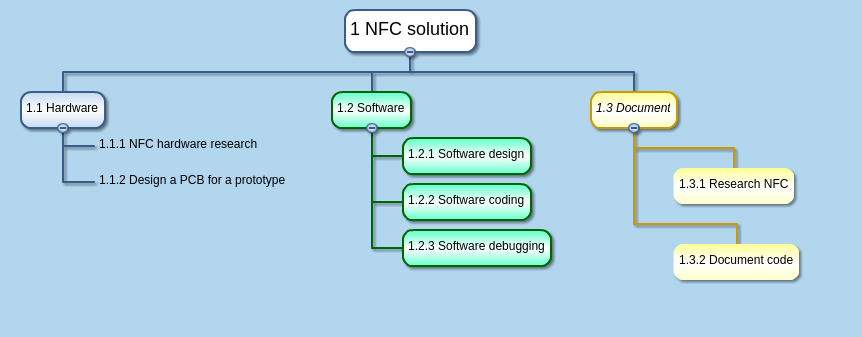
\includegraphics[scale=0.6]{Illustrations/WBS.png}  
\caption{WBS for project}
\end{center}
\end{figure}

\section{Progress plan}
\begin{figure}[h]
\begin{center}
\center
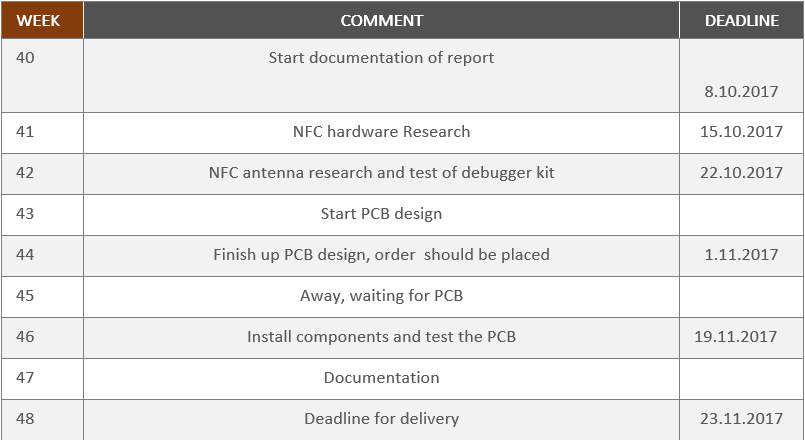
\includegraphics[scale=0.6]{Illustrations/work_plan.png}  
\caption{Progress plan}
\end{center}
\end{figure}


\end{appendices}


